
\chapter{Constructing hardware with \cf HDL}
\label{chap:CAFEO}
%~~~~~~~~~~~~~~~~~~~~~~~~~~~~~~~~~~~~~~~~~~~~~~~~~~~
\section{Introduction}
%~~~~~~~~~~~~~~~~~~~~~~~~~~~~~~~~~~~~~~~~~~~~~~~~~~~

\paragraph{}\cf HDL and compiler are specifically tailored to handle the limitations we discussed in \autoref{chap:motivation}. Their main features include:
\begin{itemize}
\item Intuitive dataflow programming.
\item Bit-accurate operations including bit aliasing.
\item Full object-oriented support including inheritance, type safety, operator overloading, and polymorphism.
\item Constraints programming (OscaR\cite{team3258oscar}-based).
\item Device-agnostic and timing-agnostic design.
\item Software (Scala-based) backend, which enables the designer to run and debug code easily within the Scala integrated development environment (IDE).
\item Hardware (Chisel\cite{bachrach2012chisel}-based) backend that compiles the design to an RTL verilog code.
\end{itemize}

\begin{figure*}[htb]
  \centering
  \includegraphics[width=0.65\textwidth]{graphics/CAFEO_Design_Flow.pdf}
  \caption{\cf design flow}\label{fig:CAFEO design flow}
\end{figure*}
%~~~~~~~~~~~~~~~~~~~~~~~~~~~~~~~~~~~~~~~~~~~~~~~~~~~


%~~~~~~~~~~~~~~~~~~~~~~~~~~~~~~~~~~~~~~~~~~~~~~~~~~~
\section{From HDL limitations to \cf HDL}
%~~~~~~~~~~~~~~~~~~~~~~~~~~~~~~~~~~~~~~~~~~~~~~~~~~~
\paragraph{}Following the discussion in \autoref{chap:motivation}, we conclude that a proper HDL needs to be device-agnostic and timing-agnostic, so a design's functionality need only be validated once and not for every target. We also conclude that it is not necessary for the HDL to be concurrent, and in fact, this often makes it more difficult to construct hardware. 
\paragraph{}We note that a trait common to all hardware designs is dataflow (DF). DF programming is used when we wish to describe the hardware stages the data will flow through without specifying specific timing or which logic technology is used (\autoref{sec:limitation synchronous}). Concurrency (\autoref{sec:limitation_concur}) is assumed and only a DF connection can trigger DF chaining (sequential operations). DF also assumes that the data is valid, thus solves the abstraction required by \autoref{sec:limitation invalid}. Additionally, we require the DF to be bit accurate (\autoref{sec:limitation bit-accuracy}).
\paragraph{}We wanted advanced object oriented capabilities, and a functional language with operator overloading and type-safety to create a new type system to support the bit-accurate DF requirements. Scala is functional and has the language properties we were looking for.  

\paragraph{}Chisel is an HDL based on Scala. As specified in \autoref{chap:relwork}, Chisel falls short of characteristics we require from a proper HDL, but it was an appropriate choice for a backend to generate the hardware for synthesis. This saved us time to from directly translating \cf code into hardware. Furthermore, \cf can bridge to Chisel, which provides a top-level IO interface. This saved us time from adding this language construct to \cfns. 

\paragraph{}Using Scala's rich type system, we created expandable DF types to handle bit-accurate operations including bit concatenation and range selection. We added constraints programming mechanism (\autoref{sec:limitation separate contraints}) to \cf using OscaR \cite{team3258oscar}, a constraints programming solver library for Scala.
%~~~~~~~~~~~~~~~~~~~~~~~~~~~~~~~~~~~~~~~~~~~~~~~~~~~


\newpage
%~~~~~~~~~~~~~~~~~~~~~~~~~~~~~~~~~~~~~~~~~~~~~~~~~~~
\section{Coding with \cf}
%~~~~~~~~~~~~~~~~~~~~~~~~~~~~~~~~~~~~~~~~~~~~~~~~~~~
\label{sec:Coding with CAFEO}
%---------------------------------------
\subsection{General example}
%---------------------------------------
\paragraph{}\cf is a Scala library and adds types and definitions to enable the dataflow (DF) programming paradigm described in \autoref{sec:df_prog_paradigm}. \cfns's code simplicity is demonstrated in \autoref{fig:General example code}. The code defines a Scala function that accepts and returns a single DF bits vector. It uses only 8 bits of \textit{In8} and outputs a 16 bits vector (\textit{bits16}). \cf will automatically zero-extend \textit{In8} if it is narrower than 8 bits or use its least significant bits if it is wider (compilation warning or error assertions can be added to check for \textit{In8}'s width).

\begin{figure*}[h]
	\centering
	\begin{minted}[linenos,tabsize=2,gobble=2,frame=single,framesep=5pt]{Scala}
		def exampleFunc(In8 : DFBitsLike) : DFBitsLike 
		{
			val bits16 = DFBitsVar(16) //creating a 16-bits DF var
			val my_byte_alias = bits16(15,8) //aliasing most significant byte
			bits16(7,0) := In8 //assigning In8 to 8 least significant bits
			bits16(15,8) := In8 + 3  //assigning In8+3 to 8 most significant bits
			val my_bits_alias = my_byte_alias(4,3) //aliasing two bits
			ifdf (bits16(4)) { //conditioned according to In8, bit #4
				my_bits_alias := 0 //clearing bits16's 11,12 bits via aliasing, 
			}                    //conditionally dependent on In8, bit #4
			bits16(7,4) := 0 //clearing bits 7,6,5,4
			bits16 := bits16 - 1 //subtracting 1 from bits16 var as a whole
			return bits16
		}
	\end{minted}
	\caption{General example code}\label{fig:General example code}
\end{figure*}

\paragraph{}The code in \autoref{fig:General example code} demonstrates several features of \cfns's coding style: 
\begin{itemize}
	\item Variable reassignment (lines 5, 6, 9, 11 and 12). See \autoref{subsec:var_assign}.
	\item Bit aliasing (lines 4, 5, 6, 7, 9 and 11). See \autoref{subsec:bit_alias}.
	\item Conditional clauses (lines 8--10). See \autoref{subsec:cond_clause}.
	\item Operators (lines 6 and 12). See \autoref{subsec:operators}.
	\item Auto pipelining and fork-join (lines 6, 8--10 and 12). See \autoref{subsec:auto_pipelining} and \autoref{subsec:auto_fork-join}.
\end{itemize}
%---------------------------------------


\newpage
%---------------------------------------
\subsection{Variable (re)assignment}
%---------------------------------------
\label{subsec:var_assign}
\paragraph{}DF variable assignment in \cf is very similar to variable assignment in VHDL. In our general example (\autoref{fig:General example code}) the DF variable \textit{bits16} can be reassigned to again and again either in part (lines 5,6,9, and 11) or as a whole (line 12). Assignments to different bits are independent (e.g., lines 5,6), while reassignment to the same bits causes the latest assignment to be used when these bits are read (\textit{ifdf} condition in line 8 uses assignment from line 4, while subtraction operation in line 12 uses all the latest assignments). All partial variable referencing such as in lines 5\&6 use the bit aliasing mechanism, which is described next, in \autoref{subsec:bit_alias}.
\paragraph{}\autoref{fig:Switch vars function code} illustrates another example of variable assignment. It shows how to switch data between two DF bits variables. Unlike native HDLs, it is required to use a temporary variable to switch between values, since the dataflow is changed immediately after every assignment. It is important to note that this function generates no hardware, since no hardware is constructed from assignments (performance reduction may manifest in longer compilation time only). 
\begin{figure*}[h]
	\centering
	\begin{minted}[linenos,tabsize=2,gobble=2,frame=single,framesep=5pt]{Scala}
		def switchBitsVars(a : DFBitsVarLike, b : DFBitsVarLike) : Unit
		{
			assert(a.width == b.width) //generate error for mismatched width
			val temp = DFBitsVar(a.width) //creating a temporary variable
			temp := a //save value of a
			a := b //copy value of b
			b := temp //copy value of a, stored by temp
		}
	\end{minted}
	\caption{Switch vars function code}\label{fig:Switch vars function code}
\end{figure*}
\paragraph{}\cf differentiates between DF-mutable (Var) and DF-immutable (Val) variables within its type system. Since both \textit{a} and \textit{b} are of a \textit{DFBits\textbf{Var}Like} type, they can accept the ':=' assignment operator and therefore be modified by the function (more on \cfns's type system in \autoref{sec:type_system}). 
\paragraph{}Each variable in \cf has a constant width, either defined explicitly by a designer instantiated constructor (line 4) or implicitly by a logical/mathematical operation (see \autoref{subsec:operators}). Assignment between different width variables is possible in \cfns, when using the standard \textit{DFBits***Like} types. \cf is type-safe (thanks to Scala's type-safety), but enables the designer some leeway to create new types and generic functions with ease and without unnecessary warnings. Type safety can be enforced either by using different types in Scala, or using \cfns's compiler, as demonstrated in line 3 in the example above (warnings/errors can also be enabled by default and exceptions made at specific code regions for stricter type enforcement). 


%---------------------------------------

%---------------------------------------
\subsection{Bit aliasing}
%---------------------------------------
\label{subsec:bit_alias}
\paragraph{}\cf enables referencing part of a DF variable using a new variable which acts as a 'bits pointer', meaning all changes to one will affect the other (similar to VHDL's signal aliasing). Aliasing a DF alias variable is also possible, maintaining relative bits numbering. \autoref{fig:Aliasing example} shows  the potential effect of aliasing on a DF variable's data (\textit{bits128}).
\begin{figure*}[h]
	\centering
	\begin{subfigure}[b]{0.49\textwidth}
		\begin{minted}[linenos,tabsize=2,gobble=3,frame=single,framesep=5pt]{Scala}
			val bits128 = DFBitsVar(128)
			val alias64 = bits128(127, 64)
			val alias32 = alias64(31, 0)
			alias32(16, 8) := 0x57		    
		\end{minted}
		\caption{Code}
		\label{fig:Aliasing code}
	\end{subfigure}%
	\hfill
	\begin{subfigure}[b]{0.49\textwidth}
		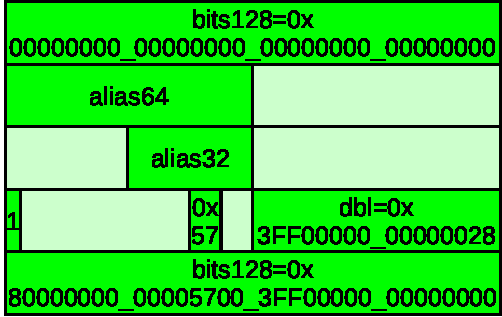
\includegraphics[width=1.0\linewidth]{graphics/Aliasing.pdf}
		\caption{Data}
		\label{fig:Aliasing data}
	\end{subfigure}
	\caption{Aliasing example}\label{fig:Aliasing example}
\end{figure*}
\paragraph{}\cfns's code safety is enforced by maintaining the 'DF-mutability' trait while aliasing (accepting the ':=' operator). This means that an alias of a \textbf{Var}, is still a \textbf{Var}, and can be assigned, while an alias of a \textbf{Val} cannot. This concept is illustrated in \autoref{fig:Aliasing Vars vs Vals}, and further explained in \autoref{sec:type_system}:
\begin{figure*}[h]
	\centering
	\begin{minted}[linenos,tabsize=2,gobble=2,frame=single,framesep=5pt]{Scala}
		val bits32 = DFBitsVar(32) //define 32 bits DF variable
		val bits8 = bits32(7, 0)   //alias 8 least significant bits 
		val adder32 = bits32 + 1   //save reference to adder
		val adder8 = adder32(7, 0) //alias 8 least significant bits of the 
		                           //adder
		bits32  := 1 //possible (Var assignment)
		bits8   := 1 //possible (Alias of Var is a Var)
		adder32 := 1 //error (operator ':=' not available)
		adder8  := 1 //error (operator ':=' not available)
		bits32  := adder32 //possible (adder32 can be read)
	\end{minted}
	\caption{Aliasing \textbf{Var} vs \textbf{Val}}\label{fig:Aliasing Vars vs Vals}
\end{figure*}

\paragraph{}Bit aliasing is also usable across different DF variable types to allow casting. Every DF type has a \textit{.bits(Hi,Lo)} and \textit{.bit(num)} methods that return an alias of a DFBits or DFBool types, respectively. Its purpose is to be used mostly when creating new types and not to blindly cast between one type to another. More on this in \autoref{sec:type_system}, where we specify \cfns's type system.
%---------------------------------------

 
%---------------------------------------
\subsection{Nested conditional clauses}
%---------------------------------------
\label{subsec:cond_clause}
\paragraph{}\cf supports all nesting of \textit{ifdf} \& \textit{elseifdf} statement clauses, along with bit aliasing. These clauses are transformed into multiplexers (muxes), where each branch of the condition always exists, and the muxes select between the branches.
\begin{figure*}[h]
	\centering
	\begin{minted}[linenos,tabsize=2,gobble=2,frame=single,framesep=5pt]{Scala}
		val a = DFBitsVar(8)
		val cond1 = DFBoolVar()
		val cond2 = DFBoolVar()
		val cond3 = DFBoolVar()
		
		a := 0x10
		cond1 := 0
		cond2 := 1
		cond3 := 0
		ifdf (cond1) {
			a := 2
		}.elseifdf (cond2) {
			a := 5
			a := 7
		} elsedf {
			ifdf (cond3) {
				a := 8
			} elsedf {
				ifdf (cond1) {
					a := 3
				}
			}
		}
		assert(a.toBigInt() == BigInt(7))
	\end{minted}
	\caption{Nested conditional example code}\label{fig:Nested conditional example code}
\end{figure*}
%---------------------------------------


%---------------------------------------
\subsection{Auto pipelining}
%---------------------------------------
\label{subsec:auto_pipelining}
\paragraph{}Any logic operation takes minimum delay time from stable input to stable output. For synchronous logic that minimum time between any two registers sets the maximum frequency possible to operate the logic clock without errors. \cf receives the required maximum delay and places registers automatically to limit the maximum delay accordingly. Furthermore, each register adds latency. \cf adds registers to balance the input latencies of binary operations in order to maintain functional correctness. 
%---------------------------------------


%---------------------------------------
\subsection{Auto fork-join, ready-valid dependencies}
%---------------------------------------
\label{subsec:auto_fork-join}
\paragraph{}\cf automatically places ready-valid handshake logic for all added registers, molding them into a small pipelined fifo. All operations which take more than one input have their ready-valid handshake signals joined. Each value that is used by more than one operation has its ready-valid handshake signals forked.
%---------------------------------------


%---------------------------------------
\subsection{Operators}
%---------------------------------------
\label{subsec:operators}
\paragraph{}\cf supports multiple unsigned bits and boolean operations (but only operations necessary for this research were implemented). The following bits operations are supported: Xor ($^\wedge$), Or ($\vert$), And (\&), Not ($\backsim$), Left Shift ($<<$), Right Shift ($>>$), Equals (==), Not Equals (!=), Bit Concatenation (\#\#), Add (+), Subtract (-), Multiply (*). The following boolean operations are supported: Xor ($^{\wedge\wedge}$), Or ($\vert\vert$), And (\&\&), Not (!)
%---------------------------------------
%~~~~~~~~~~~~~~~~~~~~~~~~~~~~~~~~~~~~~~~~~~~~~~~~~~~

\newpage
%~~~~~~~~~~~~~~~~~~~~~~~~~~~~~~~~~~~~~~~~~~~~~~~~~~~
\section{\cfns's dataflow programming paradigm}
%~~~~~~~~~~~~~~~~~~~~~~~~~~~~~~~~~~~~~~~~~~~~~~~~~~~
\label{sec:df_prog_paradigm}

%---------------------------------------
\subsection{Execution views}
%---------------------------------------
\paragraph{}Explicit concurrent coding limitation, as discussed in \autoref{sec:limitation_concur}, applies to all HDLs that have been declared as concurrent (such as Vivado HLS, Cx, MyHDL, Chisel, Bluespec, etc.). Concurrency does not need to be explicit, but can be derived from the dataflow. That is why designing hardware in \cf is very similar to a single threaded software programming, as \cf aims for sequential and intuitive code design (with several enhancements such as bit-accuracy and aliasing). The key difference is that the execution flow does not follow conventional software execution.
We will explain this further using the following diagram:
\begin{figure*}[h]
  \centering
  \includegraphics[width=0.85\textwidth]{graphics/DF_Paradigm_basic.pdf}
  \caption{DF programming paradigm}\label{fig:DF_Paradigm_basic}
\end{figure*}
\paragraph{}\autoref{fig:DF_Paradigm_basic} illustrates two independent dataflows, A and B, which are used by the flow C. The A and B flows are mixed together, while C flow is naturally executed last, since it uses references from both A and B (notice the difference from concurrent coding, where the C flow could have been listed anywhere). 

Code in \cf can be executed by one of two backends with different code views, while maintaining functional correctness (same results in both backends):
%Concurrency is required for verification, but in our view, it should be considered as a different tools
\begin{itemize}
	\item Software-level simulation backend: The entire DF code is execute sequentially, as written, leading to the same execution view as the code view (top$\rightarrow$bottom), as can be seen from the figure. More on this in \autoref{subsec:software_backend}.
	\item Synthesizable RTL backend: The hardware is \textbf{constructed serially} for maximum \textbf{parallel execution}, while constrained by DF dependency. As demonstrated by the figure, the execution view of the hardware backend has two parallel flows of A and B, which converge into C, due to DF dependency constraints. More on this in \autoref{subsec:hardware_backend}.
\end{itemize}
%---------------------------------------

%---------------------------------------
\subsection{Software backend: Simulation and debugging}
%---------------------------------------
\label{subsec:software_backend}
\paragraph{}The software backend helps us check for mathematical/logical errors simply, quickly and early in the design flow. The compiler calculates values of the DF variables as it passes through the code serially. By using the Scala IDE, the designer can debug the code as a step-by-step process, use watches, printout to console, access files, etc.  

\paragraph{}Although it provides a simple check, this backend's coverage potential is profound, due to correctness guarantees of the DF. An optional debug loop can be used to inject new test inputs and propagate data through the DF. It is important to note that the order of inputs injections remains the same through all the loops (executed \textit{as-written}), which is why further coverage is required when thoroughly verifying the hardware implementation.

\paragraph{}It is important to note that the \cf compiler requires rerunning the DF code for every new input data we wish to inject, inherently re-instantiating all the DF elements and purging any DF propagation state. Resolving this, as well as supporting \textit{State} in general, is a matter for future work (see \autoref{chap:conclusion}).
%---------------------------------------

%---------------------------------------
\subsection{Hardware backend: Synthesizable RTL generation}
%---------------------------------------
\label{subsec:hardware_backend}
\paragraph{}The hardware backend enables us to create synthesizable constructs by compiling the DF code to a low level HDL code (verilog) and constraints files. The order of the hardware's construction is sequential, but independent paths are constructed as different hardware logic paths, hence executed concurrently in hardware. The compiler adds all required logic to allow for paths to be joined, forked, pipelined and latency balanced, while maintaining functional correctness to match the software backend's results (more on this in \autoref{chap:Compiler}). 

\paragraph{}Note that the backend creates synchronous code. As established in \autoref{chap:motivation} the DF code is device and timing agnostic, meaning correctness can be maintained for any type of timing or device, including asynchronous design topology, multiple clock domains, etc. All these features have yet to be explored, and are left for future work.
%---------------------------------------

%---------------------------------------
\subsection{Paradigm characteristic - Pseudo out of order execution}
%---------------------------------------
\paragraph{}As we first mentioned in this section, coding in \cf is similar to software coding, as well as testing it within the IDE. However, execution in hardware can be out of order, to provide maximum concurrency within the DF constraints. DF paths which are independent of one another can be executed in parallel, and therefore constructed accordingly by the \cf compiler.

\paragraph{}\autoref{fig:Pseudo ooo example} shows example of two identical code segments except for the swapped lines 5 and 6. Since the DF vars \textit{a} and \textit{b} have separate DF paths, and swapping the lines changes nothing within those paths, the codes compile to the same hardware construction (note that an execution using the software backend will result in the same final value of \textit{c}, but differs in execution order to match the written expressions' order).
\begin{figure*}[h]
	\centering
	\begin{subfigure}[b]{0.30\textwidth}
		\begin{minted}[linenos,tabsize=2,gobble=3,frame=single,framesep=5pt]{Scala}
			//a, b and c are 
			//DFBitsVar vars
			//
			a := a & 0x3F
			b := b + 1
			a := a - 5
			b := b ^ 0x3
			c := a + b
		\end{minted}
		\caption{Code option 1}
		\vspace*{4mm}
	\end{subfigure}%
	\hfill
	\begin{subfigure}[b]{0.32\textwidth}
		\includegraphics[width=1.1\textwidth]{graphics/DF_out_of_order.pdf}
		\caption{Hardware dataflow}
		\vspace*{4mm}
	\end{subfigure}%
	\hfill
	\begin{subfigure}[b]{0.30\textwidth}
		\begin{minted}[tabsize=2,gobble=3,frame=single,framesep=5pt]{Scala}
			//a, b and c are 
			//DFBitsVar vars
			//
			a := a & 0x3F
			a := a - 5
			b := b + 1
			b := b ^ 0x3
			c := a + b
		\end{minted}
		\caption{Code option 2}
		\vspace*{4mm}
	\end{subfigure}
	\caption{Pseudo out of order execution code example}\label{fig:Pseudo ooo example}
\end{figure*}
%---------------------------------------

%---------------------------------------
\subsection{Paradigm characteristic - Pseudo function inlining}
%---------------------------------------
\paragraph{}Scala methods for DF variables are non-constricting in matters of hardware execution order. The latter is constrained solely by the path of the DF variables operations. Consequently, Scala methods serve more of an inner scope encapsulation for the DF programming paradigm, an important role on its own. This enables finite recursions and any object oriented capabilities of the Scala language. This means we can freely use functional hierarchies, and the hardware construction shall remain unaffected (only can be longer compilation times for both hardware and software views).

\paragraph{}\autoref{fig:Pseudo function inlining example} shows two code examples which produce the same hardware. The code on the right possesses a method which accepts two variables, \textit{a} and \textit{b}, but only uses \textit{a}, meaning the \textit{b} variable can be modified in parallel to the \textit{a}. The method is not blocked until \textit{b} value is ready, and \textit{b} operations do not wait for the method to be return.
\begin{figure*}[h]
	\centering
	\begin{subfigure}[b]{0.29\textwidth}
		\begin{minted}[linenos,tabsize=2,gobble=3,frame=single,framesep=5pt]{Scala}
			//a, b and c are 
			//DFBitsVar vars
			//
			a := a & 0x3F
			b := b + 1
			a := a - 5
			b := b ^ 0x3
			c := a + b
		\end{minted}
		\caption{Option code 1}
		\vspace*{4mm}
	\end{subfigure}%
	\hfill
	\begin{subfigure}[b]{0.69\textwidth}
		\begin{minted}[tabsize=2,gobble=3,frame=single,framesep=5pt]{Scala}
			def modA(a : DFBitsVarLike, b : DFBitsVarLike) {
				a := a & 0x3F
				a := a - 5
			}
			b := b + 1
			modA(a, b)
			b := b ^ 0x3
			c := a + b
		\end{minted}
		\caption{Option code 2}
		\vspace*{4mm}
	\end{subfigure}
	\caption{Pseudo function inlining code example}\label{fig:Pseudo function inlining example}
\end{figure*}
%---------------------------------------

%---------------------------------------
\subsection{Paradigm characteristic - Pseudo loop unrolling}
%---------------------------------------
\paragraph{}Loops in \cf are used to repeat construction steps and are inherently unrolled at compile time. The concept is similar to generation loops in VHDL. Iterative DF variables assignments can construct either sequential or concurrent hardware, depending on the formed DF paths. Non-DF Scala variables act the same as always. The loops have to be finite (or else the construction will never end, causing the compilation to hang).
\paragraph{}\autoref{fig:Pseudo loop unrolling example} demonstrates a \textit{for} loop in \cfns. The non-DF variable \textit{i} is updated at every iteration of the loop and effects the constant value in the addition operations of the DF variables \textit{a} and \textit{b}. Though the operation is the same, the \textit{b} additions result in a sequential operation, due to DF dependency, while the \textit{a} operations are constructed concurrently, due to independent aliased sections of \textit{a}.
\begin{figure*}[h]
	\centering
	\begin{subfigure}[b]{0.49\textwidth}
		\begin{minted}[linenos,tabsize=2,gobble=3,frame=single,framesep=5pt]{Scala}
			//a,c are 32bits DFBitsVar vars
			//b is an 8bits DFBitsVar vars
			for (i <- 0 until 4) {
				val byteA = a((i+1)*8-1, i*8)
				byteA := byteA + (i + 1)
				b := b + (i + 1)
			}
			c := a + b
		\end{minted}
		\caption{Code}
		\vspace*{2mm}
	\end{subfigure}
	\hfill
	\begin{subfigure}[b]{0.44\textwidth}
		\includegraphics[width=1.0\linewidth]{graphics/DF_loop_unrolling.pdf}
		\caption{Hardware dataflow}
		\vspace*{2mm}
	\end{subfigure}
	\caption{Pseudo loop unrolling code example}\label{fig:Pseudo loop unrolling example}
\end{figure*}
%---------------------------------------

\newpage
%---------------------------------------
\subsection{Paradigm characteristic - Pseudo conditional execution clauses}
%---------------------------------------
\paragraph{}\cfns's \textit{ifdf} clauses translate into multiplexers for DF variables. Unlike normal \textit{if-else} conditioning, all clauses are executed and not just the \textit{true} clause and they accept only DF boolean conditions. This causes all non-DF Scala variables within these clauses to be updated as if they weren't under \textit{if} conditioning at all, because they are actually not. While this seem counter-intuitive at first, it provides a very clear coding separation between DF paths and software paths. Scope encapsulation within each \textit{ifdf} clause is the same as any Scala program.
\paragraph{}\autoref{fig:Pseudo conditional execution clauses example} demonstrates how a Scala non-DF variable \textit{test} is unaffected by the \textit{ifdf} clauses' conditioning and is incremented freely at lines 5, 8, 11 and 14. On the other hand, the DF variable \textit{a} is muxed according to the conditioning and uses the updated \textit{test} at each clause. As can be seen from the hardware dataflow illustration, the \textit{ifdf} selects \textit{a} to be one of \textit{\{a, a+1, a+2, a+3, a+4\}} values.
\begin{figure*}[h]
	\centering
	\begin{subfigure}[b]{0.7\textwidth}
		\begin{minted}[linenos,tabsize=2,gobble=3,frame=single,framesep=5pt]{Scala}
			//a is a DFBitsVar var
			//c1-3 are a DFBoolVar vars
			var test = 0	
			ifdf (c1) {
				test = test + 1
				a := a + test
			}.elseifdf (c2) {
				test = test + 1
				a := a + test
			}.elseifdf (c3) {
				test = test + 1
				a := a + test
			} elsedf {
				test = test + 1
				a := a + test
			}
		\end{minted}
		\caption{Code}
		\vspace*{4mm}
	\end{subfigure}
	\vfill
	\begin{subfigure}[b]{0.80\textwidth}
		\includegraphics[width=1.0\linewidth]{graphics/DF_conditional_execution.pdf}
		\caption{Hardware dataflow}
		\vspace*{4mm}
	\end{subfigure}
	\caption{Pseudo conditional execution clauses code example}\label{fig:Pseudo conditional execution clauses example}
\end{figure*}
%---------------------------------------
%~~~~~~~~~~~~~~~~~~~~~~~~~~~~~~~~~~~~~~~~~~~~~~~~~~~



\newpage
%~~~~~~~~~~~~~~~~~~~~~~~~~~~~~~~~~~~~~~~~~~~~~~~~~~~
\section{\cfns's type system}
%~~~~~~~~~~~~~~~~~~~~~~~~~~~~~~~~~~~~~~~~~~~~~~~~~~~
\label{sec:type_system}
%---------------------------------------
\subsection{\cf Scala libray}
%---------------------------------------

\paragraph{}\cf is a Scala library. Hence, it inherently supports Scala's very own rich and powerful type system. \cf adds new types to support its bit-accurate DF programming paradigm, as detailed in \autoref{sec:df_prog_paradigm}. 

\paragraph{}\autoref{fig:CAFEO dataflow type classes} illustrates the inheritance hierarchy of the main DF type traits, abstract classes, and classes. Generic types are colored in green. All other DF types are derived from these. An example of a standard general purpose Bits type hierarchy is colored in yellow. 

\begin{figure*}[htb]
  \centering
  \includegraphics[width=1.0\textwidth]{graphics/Classes.pdf}
  \caption{\cf dataflow type classes \& inheritance}\label{fig:CAFEO dataflow type classes}
\end{figure*}

\paragraph{Generic DF traits}Every DF variable must be a descendant of the DFAnyLike trait. %(\autoref{subsec:DFAnyLike trait})
Variables of this type \underline{alone} are DF-immutable, meaning they cannot accept new DF assignments. An immediate descendant of this trait is the DFAnyVarLike %(\autoref{subsec:DFAnyVarLike trait}) 
trait which adds DF-assignability, turning all descendants of it to DF-mutable variables.

\paragraph{Generic DF abstract classes}Every instantiated DF class variable must be one of the following four abstract classes' descendant: 
\begin{itemize}
	\item DFAnyA - Usually created as a result of an operation between two DF types or when casting  one DF type to another. Variables of this type are DF-immutable and cannot be assigned to (similar to Rvalues in C), thus contain a single value representation for each bit.
	\item DFAnyAliasA - Variables of this type represent aliasing of DF-immutable types. DFAnyAlias points to a DFAnyLike type (or a part of it by selecting specific range of bits), which means that by reading a value of DFAnyAliasA we read from the referenced DFAnyLike. When creating a DFAnyAliasA to point to a DFAnyAliasA type, the relative bit range is translated to absolute bit range to reference the final DFAnyLike variable.
	\item DFAnyVarA - Variables of this type are DF-mutable and can be (re)assigned to (usually using ':=' operation). These variables can have multiple value representations per bit, due to additional DF scopes created by conditional assignments in 'ifdf' clauses. When a scope is no longer required it is converged into a mux oper
	\item DFAnyAliasVarA - Variables of this type represent aliasing of DF-mutable types. Although the aliasing concept is similar to DFAnyAliasA, the DFAnyAliasVarA variables reference DFAnyVarLike types only. In short- an alias of a DF-mutable variable is DF-mutable; An alias of DF-immutable variable is DF-immutable.
\end{itemize}

%%---------------------------------------
%\subsection{DFAnyLike trait}
%%---------------------------------------
%\label{subsec:DFAnyLike trait}
%\Q{the ':=' operator is not present and will cause an error viewable by the IDE }
%%---------------------------------------
%
%%---------------------------------------
%\subsection{DFAnyVarLike trait}
%%---------------------------------------
%\label{subsec:DFAnyVarLike trait}
%%---------------------------------------


\begin{figure*}[t]
	\centering
	\begin{minted}[tabsize=2,gobble=2,frame=single,framesep=5pt]{Scala}
		//Only public definitions are displayed
		trait DFAnyLike { 
			val width : Int
			def bits(bitHigh : Int = width-1, bitLow : Int = 0) : BITS
			def bit(bit : Int) : BOOL
		}
		trait DFAnyVarLike[-VAL <: DFAnyLike] extends DFAnyLike {
			def := (that : VAL)
		}
	\end{minted}
	\caption{DFAnyLike \& DFAnyVarLike traits code}\label{fig:DF father traits}
\end{figure*}

%\paragraph{Width.} Every DF type has a width field defining the number of bits it posses. This value is constant, set during instantiation, since hardware construction is constant (remember- \cfns, though very similar, is not software programming but hardware construction). The maximum width is virtually limitless\footnote{Maximum bit vector width is limited by Chisel's maximum UInt width and Scala's maximum BigInt width. Good design practices lead us far away from this limit.}.
%
%\Q{mutable, immutable, like an array, Var, val, lvalue, rvalue, input, output. In this paradigm, each DF value references one or more CFG nodes.}
%\paragraph{Bits selection} 



%~~~~~~~~~~~~~~~~~~~~~~~~~~~~~~~~~~~~~~~~~~~~~~~~~~~
\section{Case study: Advanced Encryption Standard (AES) cypher implementation}
%~~~~~~~~~~~~~~~~~~~~~~~~~~~~~~~~~~~~~~~~~~~~~~~~~~~
\paragraph{}The AES cypher algorithm is implemented in \cf as specified by the FIPS 197 standard \cite{daemen2001advanced}. The following sections illustrate how some of \cfns's features are used to easily and intuitively implement AES. 

\subsection*{Galois Field DF Byte type}
\paragraph{}At its core, AES uses Galois Field arithmetic, which has different addition and multiplication operations than Euclidean space. We used Scala's operator overloading and created new DF type traits, as can be seen in \autoref{fig:AES Byte trait}. We left some of the implementations as an example.
\begin{figure*}[h]
	\centering
	\begin{minted}[linenos,tabsize=2,gobble=2,frame=single,framesep=5pt]{Scala}
		object LookupTables {
			val sboxArr = Array(0x63,0x7c, ... ) }
			
		trait AES_ByteLike extends DFByteLike {
			def + (that : AES_ByteLike) : AES_ByteLike =
				AES_Byte(this.bits() ^ that.bits())
			def + (that : Int) : AES_ByteLike
			def * (that : Int) : AES_ByteLike
			def SBox : AES_ByteLike = 
				AES_Byte(this.bits().lookupTable(LookupTables.sboxArr))
		}
		trait AES_ByteVarLike extends DFByteVarLike[AES_ByteLike] 
		      with AES_ByteLike
	\end{minted}
	\caption{AES Byte trait}\label{fig:AES Byte trait}
\end{figure*}
\paragraph{}The addition operation supports either a constant (Scala \textit{Integer}) or another \textit{AES\_Byte}, while the multiplication operation supports only a constant. Line 6 shows how casting to and from the standard \textit{DFBits} type enables the use of a XOR operation to implement the addition of the \textit{AES\_Byte}.
\paragraph{}We have also included the \textit{SBox} function, which is a non-linear substitution table used in several byte transformations. The \textit{SBox} implementation uses \cfns's \textit{lookupTable} function. This function automatically uses the FPGA's SRAM as a read only memory (ROM) to save the table, and connect it for lookup.

\subsection*{AES\_Word and AES\_Words types}
\paragraph{}The AES algorithm uses several similar data structures, but with a different functionality: Data, Key, Key Schedule and State. The standard defines these structures as a word array where each word is composed of 4 Galois Field bytes. 
\begin{figure*}[h]
	\centering
	\begin{minted}[linenos,tabsize=2,gobble=2,frame=single,framesep=5pt]{Scala}
		trait AES_WordLike extends DFWordLike[AES_ByteLike] {
			def + (that : AES_WordLike) : AES_WordLike
			def + (that : Int) : AES_WordLike
			def SubWord() : AES_WordLike
			def RotWord() : AES_WordLike = {
				val newWord = new AES_WordVar
				for (r <- 0 until 4) {
					val newR = (r + 1) % 4
					newWord(r) := this(newR)
				}
				newWord
			}
		}
		class AES_WordVar()
		  //4 bytes per word. Big Endianess.
		  extends DFWordVarA[AES_ByteLike, AES_ByteVarLike](4, BigEndian) 
		  with AES_WordVarLike
	\end{minted}
	\caption{AES\_Word trait and class types}\label{fig:AES Word trait and class types}
\end{figure*}
\paragraph{}We extended \cfns's \textit{DFWord} and \textit{DFWords} types to create \textit{AES\_Word} and \textit{AES\_Words} respectively. \autoref{fig:AES Word trait and class types} shows an example of \textit{AES\_Word} implementation. The AES standard defines the order of the bytes within the structure as big endian. By extending from \textit{DFWord} the endianess is automatically handled. When extending, we specify the \textit{AES\_ByteLike} as the \textit{DFByte} type element for the structure.
\paragraph{}The code demonstrates how \textit{RotWord} is implemented. Take note on the use of \textit{this(newR)} to get reference of Galois Field Byte at index number \textit{newR}. Also note that this function constructs no hardware, but only changed references of the DF variables.
\paragraph{}The functional AES structures (Data, Key, Key Schedule and State) are extended from \textit{DFWords} and additional functionality implemented where needed.
 
\subsection*{AES \cf code vs. AES pseudo code}
\paragraph{}\autoref{fig:AES KeyExpansion code example} shows how we implemented the AES \textit{KeySchedule} data structure and its \textit{KeyExpansion} functionality. Alongside we show the pseudo code of \textit{KeyExpansion}.
\setalgorithmicfont{\small}
\begin{figure*}[h]
	\centering
	\begin{subfigure}[b]{0.49\textwidth}
		\begin{minted}[tabsize=2,gobble=3,frame=single,framesep=5pt, fontsize=\footnotesize]{Scala}
			class AES_KeySchedule(Nk: Int, Nb: Int, 
			  Nr : Int) extends AES_Words(Nb*(Nr+1)){
				def roundKey(round : Int): AES_RoundKey
				val Rcon = Array[Int](0x00000000, ...)

				def KeyExpansion(key : AES_Key): Unit = 
				{
					val temp = new AES_WordVar
					
					
					for (i <- 0 until Nk)
						this(i) := key(i)
					
					
					


					for (i <- Nk until Nb*(Nr+1)) {
						temp := this(i-1)
						if (i % Nk == 0)
							temp := temp.RotWord().SubWord() 
								 + Rcon(i / Nk)
						else if ((Nk > 6) && (i % Nk == 4))
							temp := temp.SubWord()
							
						this(i) := this(i-Nk) + temp

					}
				}
			}
		\end{minted}
		\caption{\cf Code}
		\vspace*{2mm}
	\end{subfigure}
	\hfill
	\begin{subfigure}[b]{0.49\textwidth}
		\begin{minted}[tabsize=2,gobble=3,frame=single,framesep=5pt, fontsize=\footnotesize]{text}
			KeyExpansion(byte key[4*Nk], 
			  word w[Nb*(Nr+1)], Nk)
			begin
				word temp
				
				i = 0
				while (i < Nk)
					w[i] = word(key[4*i], key[4*i+1], 
					  key[4*i+2], key[4*i+3])
					i = i+1
				end while
				
				i = Nk
				while (i < Nb * (Nr+1)]
					temp = w[i-1]
					if (i mod Nk = 0)
						temp = SubWord(RotWord(temp)) 
						   xor Rcon[i/Nk]
					else if (Nk > 6 and i mod Nk = 4)
						temp = SubWord(temp)
					end if
					w[i] = w[i-Nk] xor temp
					i = i + 1
				end while
				
			end
		\end{minted}
		\caption{Pseudo code reference}
		\vspace*{2mm}
	\end{subfigure}
	\caption{AES KeyExpansion code example}\label{fig:AES KeyExpansion code example}
\end{figure*}

\paragraph{}It is easy to notice the great similarity between the two codes. Most changes are due to the fact \cf code is actually simpler than the pseudo code and less verbose. We have chosen to create a more object oriented code, and defined a new class for every functionally different AES data structure. 
\paragraph{}For example, the \textit{KeyExpansion} function is global in the pseudo code, and uses array data structures for the AES Key Schedule and AES Key. On the contrary, the \cf code has both \textit{AES\_KeySchedule} and \textit{AES\_Key} DF types. \textit{KeyExpansion} was defined as a function inside the \textit{AES\_KeySchedule}.
\paragraph{}Additionally, the \cf code uses the \textit{RotWord} and \textit{SubWord} functions of the \textit{AES\_Word} type, instead of the global function used in the pseudo code.

\subsection*{Advantages of \cf AES cypher implementation}
\paragraph{}With the help of \cfns's rich library, we were able to implement AES as an object oriented and intuitive code that is very similar to the standard's pseudo code, but without global functions. In some cases the algorithm is simpler in \cfns's code than that of the standard's pseudo code.
\paragraph{}In matters of debugging it was extremely easy to debug the code step-by-step using watches and console printouts. This would have been impossible to do in native HDL languages like VHDL and Verilog. After we fixed everything to work in software debugging backend, we have compiled the design to verilog using the hardware construction backend, and everything worked in RTL simulation as well.
\paragraph{}Furthermore, the code is timing-agnostic and device-agnostic, meaning it is up to the compiler to construct the hardware fitting the non-functional requirements (throughput, latency, etc.) and any target FPGA device supported by the library. In \autoref{chap:eval} we provide evaluation results of this implementation.
%~~~~~~~~~~~~~~~~~~~~~~~~~~~~~~~~~~~~~~~~~~~~~~~~~~~
\section{Case study: IEEE-754 floating-point (FP) multiplication implementation}
%~~~~~~~~~~~~~~~~~~~~~~~~~~~~~~~~~~~~~~~~~~~~~~~~~~~
\paragraph{}The IEEE-754 FP arithmetic standard \cite{ieee2008754} does not specify implementation algorithms. We had difficulty locating detailed pseudo code of FP multiplication, which completely supports the standard (including denormalized numbers and both quiet not a number (QNaN) and signaling NaN (SNaN) value groups). Finally we settled for a double precision FP open core implemented in VHDL \cite{lundgren2014open} and used its code as a reference for the algorithm. The following sections illustrate how some of \cfns's features are used to easily and intuitively implement FP multiplication. 

\subsection*{DFDouble type}
\paragraph{}One of the main advantages \cf has is an easily expandable library. We created \textit{DFDouble}, which is expandable to handle all double precision FP operations. For the scope of this work FP multiplication was sufficient. \autoref{fig:DFDouble traits} shows partial code of \textit{DFDoubleLike} and \textit{DFDoubleVarLike}.
\begin{figure*}[h]
	\centering
	\begin{minted}[linenos,tabsize=2,gobble=2,frame=single,framesep=5pt]{Scala}
		trait DFDoubleLike extends DFAnyLike {
			val sign = bit(63)
			val exponent = bits(62,52)
			val mantissa = bits(51,0)
			
			val invalid = DFBoolVar()
			
			def * (that : DFDoubleLike) : DFDoubleLike
			
			def isZero : DFBoolLike = exponent.isZero && mantissa.isZero
			def isDenormalized : DFBoolLike
			def isNaN : DFBoolLike
			def isQNaN : DFBoolLike = exponent.isAllOnes && mantissa.msbit
			def isSNaN : DFBoolLike
			def isInfinity : DFBoolLike = exponent.isAllOnes && mantissa.isZero
			def isPositive : DFBoolLike = !sign
			def isNegative : DFBoolLike = sign
		}

		trait DFDoubleVarLike extends DFDoubleLike 
		  with DFAnyVarLike[DFDoubleLike] {
		  final def := (that : Double) : Unit = 
		  	this.bits() := CAFEO_Tools.doubleToBigIntBits(that)
		  protected[CAFEO] def setAsSNaN() : Unit = {
		    exponent.setAllBits
		    mantissa := 1
		  }
		  protected[CAFEO] def setAsQNaN()
		  protected[CAFEO] def setAsInfinity()
		  protected[CAFEO] def setAsZero() : Unit = {
		    exponent.clearAllBits
		    mantissa.clearAllBits
		  }
		}
	\end{minted}
	\caption{DFDouble traits}\label{fig:DFDouble traits}
\end{figure*}
\paragraph{}Lines 2-4 show how \cfns's aliasing is usable in this case. Sign, exponent and mantissa double precision parts are easily referenced. These references are usable both as immutable and mutable variables in \textit{DFDoubleLike} and \textit{DFDoubleVarLike} respectively.

\paragraph{}Lines 10, 13 and 15 give examples how to implement functional boolean indicators of the DFDouble variable. Lines 24-27 and 30-33 give examples how to set the DFDouble variable to special values.

\paragraph{}A notable definition appears in line 22. The ':=' assignment operator accepts by default only values of the same type as the trait \textit{DFDoubleLike} (as a result from \textit{DFAnyVarLike[DFDoubleLike]} inheritance). This additional definition enables assignment operation of a constant (Scala \textit{Double}).

\subsection*{Leading-zero counter (LZC) \cf code vs. pseudo code}
\paragraph{}Here we have another example how coding in \cf can be very similar to hardware algorithms written in pseudo code. In \autoref{fig:LZC+Shift code example} we show both \cf and pseudo \cite{muller2009handbook} code implementations of a combined LZC and shifter. This function is used in the FP multiplication implementation. 
\setalgorithmicfont{\small}
\begin{figure*}[h]
	\centering
	\begin{subfigure}[b]{0.49\textwidth}
		\begin{minted}[linenos,tabsize=2,gobble=3,frame=single,framesep=5pt]{Scala}
			def lzc_shift() = {
				val k = log2Up(this.width)
				val x = DFBitsVar(this.width)
				val d = DFBitsVar(k)
			
				x := this
				for (i <- k-1 downto 0) {
					ifdf (x.msbits(2~^i) == 0) {
						d(i) := 1
						x := x << 2~^i
					}
				}
				(d, x)
			}
		\end{minted}
		\caption{\cf Code}
		\vspace*{2mm}
	\end{subfigure}
	\hfill
	\begin{subfigure}[b]{0.49\textwidth}
		\begin{algorithm}[H]
  		\caption*{Combined leading-zero counting and shifting}
		\begin{algorithmic}
			\STATE{$k \leftarrow \left\lceil \log_2{n} \right\rceil$}
			\STATE{$x_k \leftarrow x$}
			 
			\FOR{$i = k-1$ downto $0$}
				\IF{there are $2^i$ leading zeros in $x_{i+1}$} 
				  \STATE{$d_i \leftarrow 1$}
				  \STATE{$x_i \leftarrow x_{i+1}$, shifted left by $2^i$}
				\ELSE 
				  \STATE{$d_i \leftarrow 0$}
				  \STATE{$x_i \leftarrow x_{i+1}$}
				\ENDIF
			\ENDFOR
			\STATE{return $(d, x0)$}
		\end{algorithmic}
		\end{algorithm}
		\caption{Pseudo code reference}
		\vspace*{2mm}
	\end{subfigure}
	\caption{LZC+Shift code example}\label{fig:LZC+Shift code example}
\end{figure*}

\paragraph{}In \cf the \textit{lzc\_shift} function is defined inside \textit{DFBitsLike} type to enable its usage for all DFBits variables. \textit{lzc\_shift} returns a tuple of the number of leading zeros (\textit{d}), and the left shifted bits vector that has no leading zeros (\textit{x}).

\paragraph{}The VHDL FP implementation we used as a reference (Lundgred core from opencores.org \cite{lundgren2014open}) has a different LZC implementation. First, its implementation has a separate shifter from the counter (need to left shift using the returned count when the count value is valid). Second, it has a naive implementation of the counter, as we can see in \autoref{fig:LZC VHDL implementation}.

\begin{figure*}[h]
	\centering
	\begin{minted}[linenos,tabsize=2,gobble=2,frame=single,framesep=5pt]{vhdl}
		function count_zeros_mul (signal s_vector: std_logic_vector) 
			return std_logic_vector is
			variable v_count : std_logic_vector(5 downto 0);	
		begin
			v_count := "000000";
			for i in 105 downto 52 loop
				case s_vector(i) is
					when '0' => v_count := v_count + "000001";
					when others => exit;
				end case;
			end loop;
			return v_count;	
		end count_zeros_mul;
		\end{minted}
	\caption{LZC VHDL implementation}\label{fig:LZC VHDL implementation}
\end{figure*}

\paragraph{}This VHDL implementation of the LZC has a long critical path, since it is described as 54 sequential addition and multiplexing operations. While a synthesis engine \textbf{might} be able to optimize this, we have not enabled such a feature within the \cf compiler. For this reason we used the algorithm described in \autoref{fig:LZC+Shift code example}, which creates a balanced tree expansion of multiplexers and does not require additions. 

\paragraph{}Balanced operation trees are important in \cfns, since the auto-pipeline and latency balancing mechanisms still cannot change the operation tree. Instead, these mechanisms add registers to latency-balance joined branches. More on this in the next chapter.


\subsection*{Bits addition, subtraction and multiplication}
\paragraph{}FP multiplication requires implemented bits operations of addition, subtraction and multiplication. \cf provides trivial usage of these operation by implementing them as part of the \textit{DFBitLike} type. \cf automatically uses the proper device IP cores and tunes them to match the required performance. More on this in the next chapter.

\subsection*{Advantages of \cf FP multiplication implementation}
\paragraph{}Again, just as in the case of the AES cypher implementation, \cfns's rich type library and type-safe object oriented support makes implementing FP multiplication fairly easy and intuitive (assuming we have a working algorithm as a reference).
\paragraph{}For an initial testing of the code, we used Scala's \textit{Double} type as a reference to get the right values of the multiplication operations and more specifically for the special cases which are not documented very well. In addition to testing special cases (QNaN, SNaN, Infinity, Zero, Denormalized, etc.) we used Scala to generate random Double values as test vectors. In all cases, debugging using the Scala IDE, proved as an invaluable feature.
\paragraph{}The VHDL implementation we used as a reference is neither timing-agnostic or device-agnostic. It is not timing-agnostic because it has constant critical path and pipelining. It is not device-agnostic because it specifically uses Xilinx Virtex-5 FPGA device multiplier primitives. On the contrary, \cfns's implementation is both timing-agnostic and device-agnostic, since it provides the proper abstraction for us to use. In \autoref{chap:eval} we provide evaluation results of \cfns's implementation.
